\chapter{测试评估}

在完成系统实现后,我们对系统进行功能与非功能性测试,以验证其是否符合预期,并评估其性能。
本章将详细介绍测试方法、测试结果以及性能评估。

\section{测试环境}

为了确保测试结果的准确性与可靠性,我们采用与实际部署环境相似的硬件和软件配置进行测试,~\ref{tab:hardware-env}与
~\ref{tab:software-env}分别展示了测试环境的硬件和软件配置。

\begin{table}
    \centering
    \caption{硬件环境}
    \label{tab:hardware-env}
    \resizebox{0.5\linewidth}{!}{
    \begin{tabular}{cl}
        \toprule
        类型   &  配置信息       \\
        \midrule
        CPU & 2x Intel Xeon Gold(2.90GHz,64核/128线程) \\
        GPU & 8x NVIDIA RTX 4090(24GB显存/卡)\\
        存储架构 & NUMA(2节点)\\
        驱动版本 & CUDA 12.2\\
        \bottomrule
    \end{tabular}
    }
\end{table}

\begin{table}
    \centering
    \caption{软件环境}
    \label{tab:software-env}
    \resizebox{0.5\linewidth}{!}{
    \begin{tabular}{cl}
        \toprule
        类型   &  配置信息       \\
        \midrule
        Next.js & 15.1.2 \\
        node.js & 22.14.0 \\
        Python & 3.9.21 \\
        flask & 3.1.0 \\
        客户端 & Google Chrome 135.0.7049.115 \\
        \bottomrule
    \end{tabular}
    }
\end{table}

\section{测试方法及用例}

为了全面评估系统的性能,我们对系统进行功能测试和非功能性测试。我们在客户端上使用Google Chrome浏览器进行测试,对
系统的各个功能模块执行一系列测试用例,并记录下测试结果;通过浏览器开发者工具等方式,对系统的响应速度、内存使用
情况等数据进行监测与分析。

\subsection{功能性测试}

\subsubsection{用户管理测试}

我们通过注册、登录、重置密码等操作,验证系统的用户管理模块是否正常工作并拦截不合法输入;并通过未登录时直接访问受保护页面,验证系统
是否正确进行了权限控制,测试结果如~\ref{tab:reg-test}、~\ref{tab:log-test}、~\ref{tab:rst-test}所示。

\begin{table}
    \centering
    \caption{注册测试}
    \label{tab:reg-test}
    \resizebox{0.8\linewidth}{!}{
    \begin{tabular}{cl}
        \toprule
        操作   &  结果      \\
        \midrule
        输入不合法的信息,如密码不合法或不匹配 & 系统拒绝注册,提示修改 \\
        输入合法信息后点击“获取验证码” & 邮箱收到验证码 \\
        输入错误验证码 & 系统提示验证码错误,拒绝注册 \\
        输入正确验证码并提交注册 & 注册成功并自动跳转到登录界面\\
        \bottomrule
    \end{tabular}
    }
\end{table}

\begin{table}
    \centering
    \caption{登录测试}
    \label{tab:log-test}
    \resizebox{0.8\linewidth}{!}{
    \begin{tabular}{cl}
        \toprule
        操作   &  结果      \\
        \midrule
        输入用户名与密码不匹配 & 登陆失败 \\
        输入匹配信息后点击“登录” & 登陆成功并自动跳转到主页\\
        未登录时访问结果查询与上传文件 & 弹出登陆提示 \\
        \bottomrule
    \end{tabular}
    }
\end{table}

\begin{table}
    \centering
    \caption{重置密码测试}
    \label{tab:rst-test}
    \resizebox{0.8\linewidth}{!}{
    \begin{tabular}{cl}
        \toprule
        操作   &  结果      \\
        \midrule
        输入用户名与邮箱不匹配 & 系统拒绝发送验证码 \\
        输入匹配信息后点击“获取验证码” & 邮箱收到验证码 \\
        输入错误验证码 & 系统提示验证码错误,拒绝重置密码 \\
        输入正确验证码并提交重置密码 & 重置密码成功并自动跳转到登录界面\\
        \bottomrule
    \end{tabular}
    }
\end{table}

\subsubsection{任务上传测试}

我们对任务上传的工作流进行测试,以验证上传工作流的正确性。测试结果如~\ref{tab:task-upload-test}所示。

\begin{table}
    \centering
    \caption{任务上传测试}
    \label{tab:task-upload-test}
    \resizebox{0.8\linewidth}{!}{
    \begin{tabular}{cl}
        \toprule
        操作   &  结果      \\
        \midrule
        上传非mp4格式的文件 & 拒绝上传,提示只允许上传mp4格式的文件 \\
        选择Prompt Type & 展开下拉菜单,包括文字、图片与重光照 \\
        输入不完整的Prompt & 拒绝提交Prompt,提示填写字段 \\
        点击Next按钮时字段空白或不合法 & 拒绝跳转,提示填写字段 \\
        选择Image Prompt后点击Next & 跳转到图片上传步骤 \\
        点击Cancel & 清除所有输入,返回第一步 \\
        输入完整信息后提交任务 & 任务提交成功,跳转回首页;后端添加任务 \\
        后端任务处理完成 & 邮箱收到完成通知 \\
        \bottomrule
    \end{tabular}
    }
\end{table}

\subsubsection{结果管理测试}

我们测试结果管理页面的项目重命名、删除、查看、查询等功能,以验证结果管理模块是否正常工作。测试结果如~\ref{tab:res-man-test}所示。

\begin{table}
    \centering
    \caption{结果管理测试}
    \label{tab:res-man-test}
    \resizebox{0.8\linewidth}{!}{
    \begin{tabular}{cl}
        \toprule
        操作   &  结果      \\
        \midrule
        重命名 & 允许编辑项目名称,确认后显示新的名称 \\
        根据名称查询 & 筛选出匹配的项目列表 \\
        删除项目 & 弹出确认弹窗,点击确认后项目被删除 \\
        查看项目 & 结果被下载到本地 \\
        \bottomrule
    \end{tabular}
    }
\end{table}

\subsubsection{数据统计测试}

数据统计为管理员功能,我们在管理员账号下进行测试,测试结果如~\ref{tab:stat-test}所示。

\begin{table}
    \centering
    \caption{结果管理测试}
    \label{tab:stat-test}
    \resizebox{0.8\linewidth}{!}{
    \begin{tabular}{cl}
        \toprule
        操作   &  结果      \\
        \midrule
        以非管理员访问 & 导航栏不显示数据统计栏目 \\
        以管理员访问 & 数据统计页面显示注册数量、一周内与总计上传数量 \\
        输入查询条件,包括时间或名称 & 筛选出对应的任务请求信息 \\
        点击导出csv & 导出任务信息的csv文件到本地 \\
        \bottomrule
    \end{tabular}
    }
\end{table}

\subsection{非功能性测试}

我们使用Chrome的Dev Tools中的Lighthouse来对系统进行性能分析。Lighthouse能够进行一系列的测试,包括性能、可访问性、
最佳实践、SEO(搜索引擎优化)以及PWA(渐进式Web应用)等方面的检测。

~\ref{fig:lighthouse}展示了Lighthouse的总体测试结果,结果显示,我们的系统在性能、可访问性、最佳实践方面均达到了优秀程度。
我们重点关注系统的性能,如~\ref{tab:perf-test}所示:系统在首次内容绘制(FCP)、最大内容绘制(LCP)、总阻塞时间(TBT)、累积布局偏移(CLS)与速度指数(SI)等方面均表现良好,
证明了系统在加载与使用过程中能够有较少的等待时间;另外累计布局偏移表明,系统在用户使用中能够提供较好的用户体验。

\begin{figure}
    \centering
    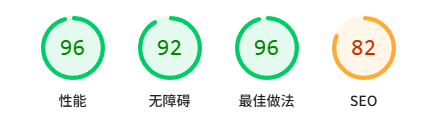
\includegraphics[width=0.6\linewidth]{source/img/lighthouse_general.png}
    \caption{Lighthouse测试结果}
    \label{fig:lighthouse}
\end{figure}

\begin{table}
    \centering
    \caption{性能测试}
    \label{tab:perf-test}
    \resizebox{0.5\linewidth}{!}{
    \begin{tabular}{cl}
        \toprule
        指标   &  结果      \\
        \midrule
        First Contentful Paint & 0.8秒 \\
        Largest Contentful Paint & 0.8秒 \\
        Total Blocking Time & 230毫秒 \\
        Cumulative Layout Shift & 0 \\
        Speed Index & 2.9秒 \\
        \bottomrule
    \end{tabular}
    }
\end{table}

\section{测试结果分析}

在上一节中,我们通过一系列测试,验证了系统的功能与实际运行性能,并取得了良好的结果。分析以上的测试,我们可以得到以下结论:
\begin{enumerate}
    \item 系统具备完整的功能,可以按照设计预期完成任务,包括用户注册、登录、任务上传、结果管理以及数据统计等功能;
    \item 系统具有较好的性能,能够在较短的时间内完成对用户操作的相应及加载,并提供稳定性较高的用户界面,提供较好的用户体验。
\end{enumerate}